%\documentclass{beamer}
%\usepackage{minijs}
%\usepackage{here}
%\mode<presentation>{
%  \usetheme{Antibes}
%  \usecolortheme{beaver}
%  \setbeamercovered{transparent}
%}
\documentclass[13pt,dvipdfmx]{beamer}
\usepackage[english]{babel}
% pdfの栞の字化けを防ぐ
\AtBeginDvi{\special{pdf:tounicode EUC-UCS2}}
% テーマ
\usetheme{metropolis}
\usepackage{caption}
\setbeamertemplate{navigation symbols}{} 
\usepackage{graphicx}
%\usepackage[dvipdfmx]{graphicx}
\usepackage{amsmath}
\usepackage{amssymb}
\usepackage{txfonts}
\usepackage{colortbl}
\usepackage{svg}
\renewcommand{\familydefault}{\sfdefault}
\renewcommand{\kanjifamilydefault}{\gtdefault}
\setbeamerfont{title}{size=\large,series=\bfseries}
\setbeamerfont{frametitle}{size=\large,series=\bfseries}
\setbeamertemplate{frametitle}[default][center]
\usefonttheme{professionalfonts} 


%1ページめ
\title{研究内容詳細}
\subtitle{クラスタリング手法の評価に向けて}
\author{池辺 颯一}
\institute{芝浦工業大学}
\date{2018年12月15日}

\begin{document}
\begin{frame}\frametitle{}
 \titlepage
\end{frame}

\begin{frame}\frametitle{概要・背景}
\begin{itemize}
 \item 情報化社会の発展によりデータが複雑かつ膨大に
 \item ビッグデータを人の手で分類するのは難しい
 \item それらのデータを自動的に分類するクラスタリングに着目
 \item 機械学習における教師なし学習にあたる
\end{itemize}
\vspace{5mm}
\begin{figure}[htbp]
 \begin{minipage}{0.4\hsize}
  \begin{center}
   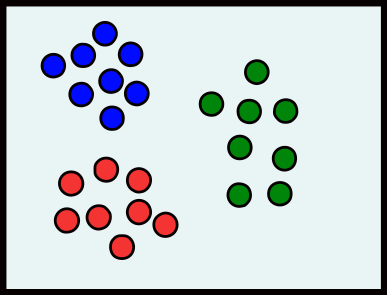
\includegraphics[width=40mm]{before_clustering.png}
  \end{center}
  \captionsetup{labelformat=empty,labelsep=none}
  \caption{クラスタリング前}
  \label{fig:one}
 \end{minipage}
\hspace{1cm}
 \begin{minipage}{0.4\hsize}
  \begin{center}
   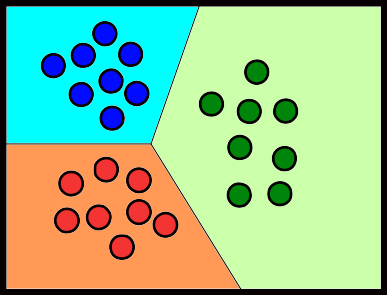
\includegraphics[width=40mm]{after_clustering.png}
  \end{center}
  \captionsetup{labelformat=empty,labelsep=none}
  \caption{クラスタリング後}
  \label{fig:two}
 \end{minipage}
\end{figure}
\end{frame}

\begin{frame}\frametitle{目的・目標}
\begin{block}{目的}
\begin{itemize}
 \item クラスタリング手法の1つであるFussy c-meansにクラスタサイズ調整変数を導入した最適化問題の中から最も精度が高いものを発見する
\end{itemize}
\end{block}
\vspace{4mm}
\begin{block}{目標}
\begin{itemize}
 \item 各クラスタリング手法のプログラムをC++を用いて開発
 \item プログラムの実行結果からクラスタリング精度を評価
\end{itemize}
\end{block}
\end{frame}

\begin{frame}\frametitle{実験対象}
  \begin{block}{既存手法}
   \begin{itemize}
    \item sFCM
    \item pFCM
    \item eFCM
   \end{itemize}
  \end{block}
 \begin{block}{提案手法}
   \begin{itemize}
    \item クラスタサイズ調整変数を導入
    \item sFCMA
    \item pFCMA
    \item eFCMA
   \end{itemize}
 \end{block}
\end{frame}

\begin{frame}\frametitle{クラスタリングの最適化問題}
  \begin{block}{eFCMA}
  \quad$\underset{u,v,\pi}{\text{minimize}}$
    $\sum_{i=1}^C\sum_{k=1}^Nu_{i,k}||x_k-v_i||_2^2+\lambda^{-1}\sum_{i=1}^C\sum_{k=1}^Nu_{i,k}\log(\frac{u_{i,k}}{\pi_{i}})$
  \end{block}
  %%  \begin{align*}
  %%   d_{i,k}&=||x_{k}-v_{i}||_{2}^2, \\
  %%   u_{i,k}&=\frac{\pi_{i}\exp(-\lambda||x_k-v_i||_2^2)}{\sum_{j=1}^C\pi_{j}\exp(-\lambda||x_k-v_j||_2^2)\quad,}\\
  %%   v_{i}=\frac{\sum_{k=1}^Nu_{i,k}x_{k}}{\quad\sum_{k=1}^Nu_{i,k}},
  %%   \alpha_{i}&=\frac{\sum_{k=1}^Nu_{i,k}}{\quad N}.
  %%  \end{align*}
  %% \end{frame}
  
  %% \begin{frame}\frametitle{クラスタリング手法}
  \begin{block}{qFCMA}
    \quad$\underset{u,v,\alpha}{\text{minimize}}$
    $\sum_{i=1}^C\sum_{k=1}^N(\alpha_{i})^{1-m}(u_{i,k})^m||x_k-v_i||_2^2$\\
    \qquad\qquad\qquad\qquad$+\frac{\lambda^{-1}}{m-1}\sum_{i=1}^C\sum_{k=1}^N(\alpha_{i})^{1-m}(u_{i,k})^m$
  \end{block}
  %%  \begin{align*}
  %%   d_{i,k}&=||x_{k}-v_{i}||_{2}^2, \\
  %%   u_{i,k}&=\frac{\alpha_{i}(1+\lambda(1-m)||x_i-v_k||_2^2)^\frac{1}{1-m}}{\quad\sum_{j=1}^C\alpha_{j}(1+\lambda(1-m)||x_j-v_k||_2^2)^\frac{1}{1-m}\quad,}\\
  %%   v_{i}=\frac{\sum_{k=1}^N(u_{i,k})^mx_{k}}{\quad\sum_{k=1}^N(u_{i,k})^{m}},
  %%  \end{align*}
  %% \end{frame}

%% \begin{frame}\frametitle{クラスタリング手法}
  \begin{block}{sFCMA}
    \quad$\underset{u,v,\alpha}{\text{minimize}}$
    $\sum_{i=1}^C\sum_{k=1}^N(\alpha_{i})^{1-m}(u_{i,k})^m||x_k-v_i||_2^2$\\
    \qquad{\text{subject to}}$\sum_{i=1}^Cu_{i,k}=1$\;,\;$\sum_{i=1}^C\alpha_{i}=1$\;and\;$u_{i,k}\in[0,1]$\quad$m>1$
  \end{block}
  %% \begin{align*}
  %%  d_{i,k}&=||x_{k}-v_{i}||_{2}^2=\left(\sqrt{\sum_{\ell=1}^m (x_{k,\ell}-v_{i,\ell})^2}\;\right)^2,\\
  %%  u_{i,k}&=\frac{1}{\sum_{j=1}^c\frac{\alpha_{j}}{\alpha_{i}}\left(\frac{d_{j,k}}{d_{i,k}}\right)^\frac{1}{1-m}},\quad
  %%  v_{i}=\frac{\sum_{k=1}^n(u_{i,k})^mx_{k}}{\quad\sum_{k=1}^n(u_{i,k})^{m}},\\
  %% \end{align*}
  \begin{itemize}
    \item $N$ : 個体数
    \item $C$ : クラスタ数
    \item $\lambda$, $m$ : ファジィ化パラメータ
    \item $u_{i,k}$ : $i$番目の個体におけるクラスタ$k$に対する帰属度
    \item $v_{i}$ : $i$番目のクラスタ中心
    \item $x_{k}$ : $k$番目の個体
  \end{itemize}
\end{frame}

\begin{frame}\frametitle{アルゴリズム}
\begin{block}{FCM(Fusssy c-means)}
\begin{enumerate}
 \item 初期クラスタ中心Vを与える
 \item Vから帰属度Uを更新する
 \item Vを更新する
 \item 収束条件を満たせば終了。満たさなければ2へ。
\end{enumerate}
\end{block}
\end{frame}

\begin{frame}\frametitle{実験方法}
\begin{center}
 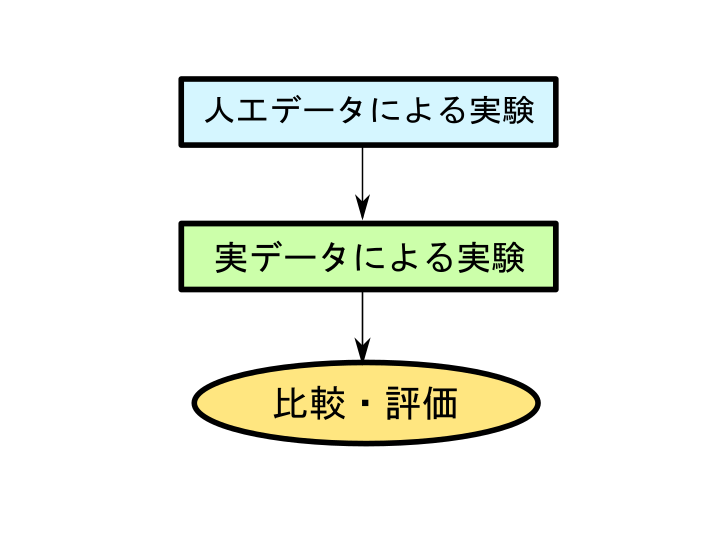
\includegraphics[width=100mm]{experiment_process.png}
\end{center}
\end{frame}

\begin{frame}\frametitle{評価方法}
\begin{block}{ARI (Adjusted Rand Index)}
\begin{itemize}
 \item -1から1までの範囲で精度評価を行う指標
 \item 1の時に完全一致で0の時にランダム
 \item マイナスの値はランダムの期待値を下回る
 \item ARIの値が高いほど高評価
\end{itemize}
\end{block}
\begin{center}
\end{center}
\end{frame}

\begin{frame}\frametitle{使用する実データ}
  \begin{block}{Yeast Data Set}
    \begin{itemize}
    \item Yeast(酵母)の形など9属性を収録したデータ
    \item ソース : UCI  Machine Learning Repository
    \item 個体数 : 1484
    \item クラス数 : 10
    \end{itemize}
  \end{block}
\end{frame}

\begin{frame}\frametitle{進捗状況}
\begin{itemize}
 \item sFCMを動作させるのに必要なプログラムを実装済
       \begin{itemize}
       \item sFCM
       \item pFCM
       \item eFCM
       \end{itemize}
\end{itemize}
\end{frame}

\begin{frame}\frametitle{課題}
\begin{itemize}
\item 処理の高速化
\item 既存手法からの継承
\end{itemize}
\end{frame}

\begin{frame}\frametitle{まとめ}
  \begin{block}{目的}
    \begin{itemize}
    \item クラスタリング手法の1つであるFussy c-meansを応用した最適化問題の中から最も精度が高いものを発見する
    \end{itemize}
  \end{block}
  \begin{block}{目標}
    \begin{itemize}
    \item 各クラスタリング手法のプログラムC++を用いて開発
    \item プログラムの実行結果からクラスタリング精度を評価
    \end{itemize}
  \end{block}
  \begin{block}{進捗}
    \begin{itemize}
    \item sFCMを動作させるのに必要なプログラムが完成
    \end{itemize}
  \end{block}
  \begin{block}{課題}
    \begin{itemize}
    \item 処理の高速化
    \end{itemize}
  \end{block}
\end{frame}

\end{document}
